\section{Numerical validations for error estimations in energy}\label{sec:numeric_energy}

In this section, we present supplementary results for the numerical validations for error estimations in electrostatic energy, complementing the main text. Figures~\ref{fig:icm_error} to~\ref{fig:error_icm_pad_gamma_1} correspond one-to-one with Figures 1 to 4 in the main text, maintaining the same systems and parameter settings as those used in the force calculation results. The dashed lines in these figures represent the fitted curves based on our theoretical estimation given in Eq.~(52) of the main text. The energy error results exhibit similar trends to the force errors and align well with our theoretical predictions.


\begin{figure}[htbp]
    \centering
    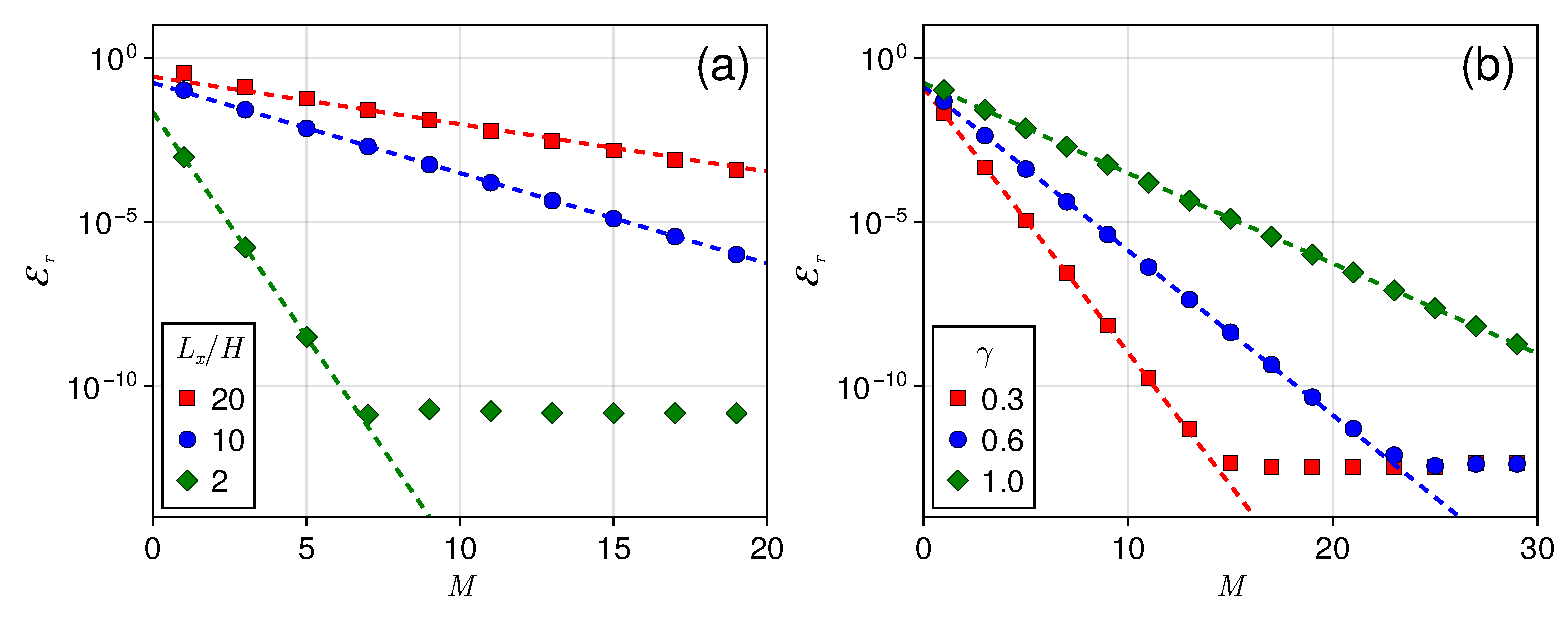
\includegraphics[width=0.98\linewidth]{figs/icm_error.pdf}
    \caption{
        Relative errors of energy due to truncation of image charges are presented. The dashed lines represent the fitted decay rate, as described in Eq. (54) in the main text. In panel (a) we set $\gamma_{\T u} = \gamma_{\T d} = 1$ and consider system heights of $H = 0.5, 1$ and $5$. In panel (b), we set $H = 1$ while varying $\gamma_{\T u} = \gamma_{\T d} = \gamma = 0.3, 0.6$ and $1$. 
        %The scope of the fitted lines are fixed to be $\lg(\gamma e^{-2\pi H / L_x})$, which is the theoretical value.
    }
    \label{fig:icm_error}
\end{figure}


\begin{figure}[htbp]
    \centering
    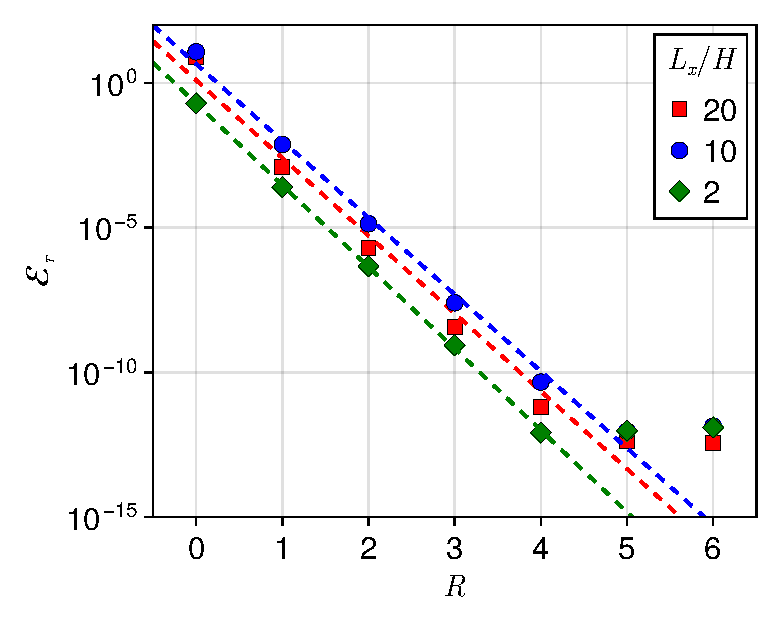
\includegraphics[width=0.49\linewidth]{figs/elc_error.pdf}
    \caption{Relative error of energy of reformulating the Ewald2D summation as 3D ones are presented. We set $\gamma_{\T u} = \gamma_{\T d} = 0$ and consider system heights of $H = 0.5, 1, 5$. Here $R = (L_z - H) / L_x$ denotes the padding ratio.}
    \label{fig:elc_error}
\end{figure}

\begin{figure}[htbp]
    \centering
    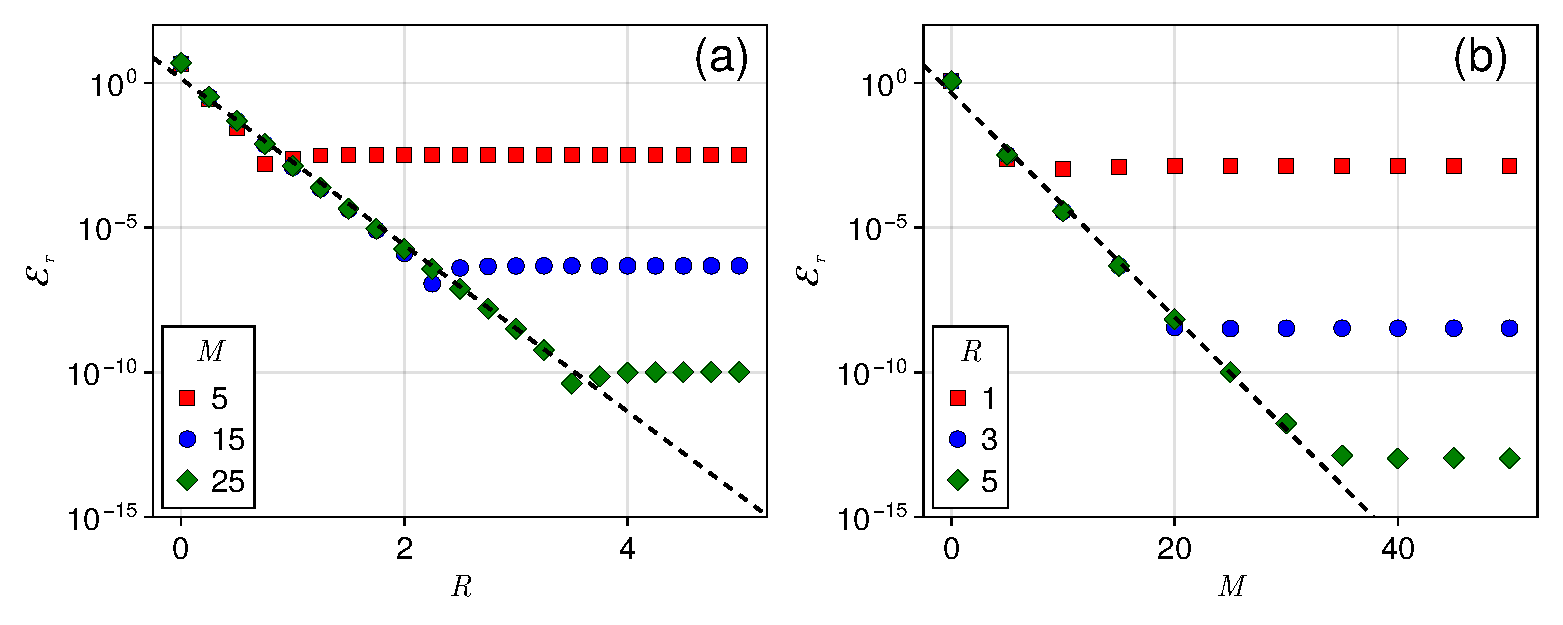
\includegraphics[width=0.98\linewidth]{figs/error_icm_pad_gamma_0.6.pdf}
    \caption{Relative error of energy in dielectric-confined Coulomb system with parameters $\gamma_{\T u} = \gamma_{\T d} = \gamma = 0.6$ and $H = 0.5$. Panel (a) illustrates error evolution with fixed image charge layers ($M = 5,~15,~25$) under varying padding ratios ($R$), whereas panel (b) demonstrates error progression with fixed $P = 1,~3,~5$ across increasing $M$.}
    \label{fig:error_icm_pad_gamma_0.6}
\end{figure}

\begin{figure}[htbp]
    \centering
    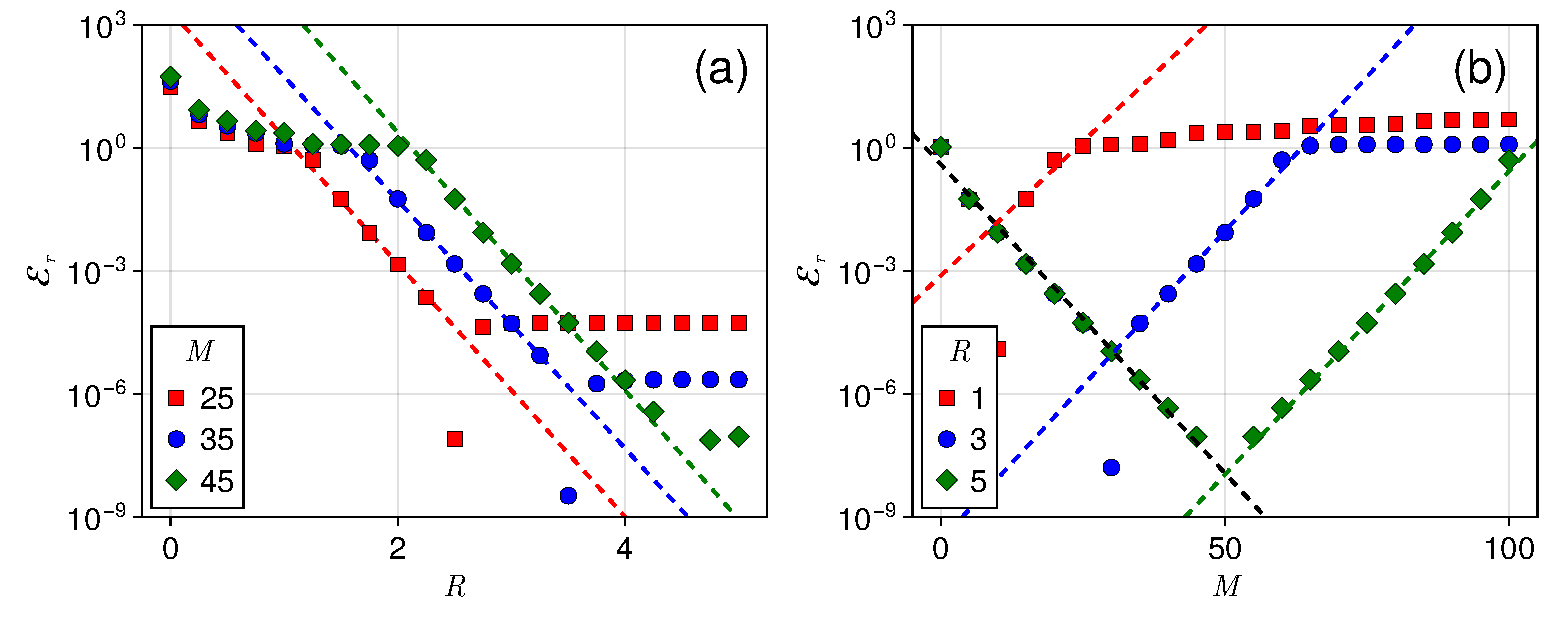
\includegraphics[width=0.98\linewidth]{figs/error_icm_pad_gamma_1.pdf}
    \caption{Relative error of energy in dielectric-confined Coulomb system with parameters $\gamma_{\T u} = \gamma_{\T d} = \gamma = 1$ and $H = 0.5$. Panel (a) illustrates error evolution with fixed image charge layers ($M = 5,~15,~25$) under varying padding ratios ($R$), whereas panel (b) demonstrates error progression with fixed $P = 1,~3,~5$ across increasing $M$.}
    \label{fig:error_icm_pad_gamma_1}
\end{figure}

\section{Challenge associated with strongly-confined systems}
In practical simulations, such as when studying thin membranes, ion transport in slit channels and supercapacitors, accurately capturing the effects of nanoconfinement, i.e., when $L_{x,y} / H\gg 1$, is crucial.
Previous numerical studies have found that more image layers are needed to achieve satisfactory accuracy for confined systems~\cite{dos2015electrolytes}. 
To further investigate the numerical properties of strongly-confined systems, we present the errors in force in Fig.~\ref{fig:icm_elc_error_force}, where we fix $L_x=L_y=10$, $R=(L_z-H)/L_x = 5$ and consider system heights $H = 0.5, 1, 5$ while varying the number of image charge layers $M$. 
In Fig.~\ref{fig:icm_elc_error_force} (a), for $\gamma = 0.6$, we observe that the error decays exponentially as $M$ increases for $H = 0.5$ and $H = 1$. 
However, for $H = 5$, where $|g_{\T u}g_{\T d}|>1$, the error becomes non-monotonic as $M$ increases, 
which is consistent with our theoretical predictions as discussed in the main text.
In Fig.~\ref{fig:icm_elc_error_force} (b), with $\gamma = 1$, we observe a similar non-monotonic pattern for all aspect ratios. 
It is important to note that, the rate of error decrease/increase depends on the aspect ratio $L_x/H$. 
A higher aspect ratio leads to a slower increase or decrease in errors, as $M$ is less or greater than the critical value that minimizes the error, respectively. 
This also highlights the computational challenge associated with strongly-confined systems -- to achieve the same accuracy, a much larger $M$ is required compared to non-confined systems.
Same conclusions hold for the errors in energy, as shown in Fig.~\ref{fig:icm_elc_error}.

\begin{figure}[htbp]
    \centering
    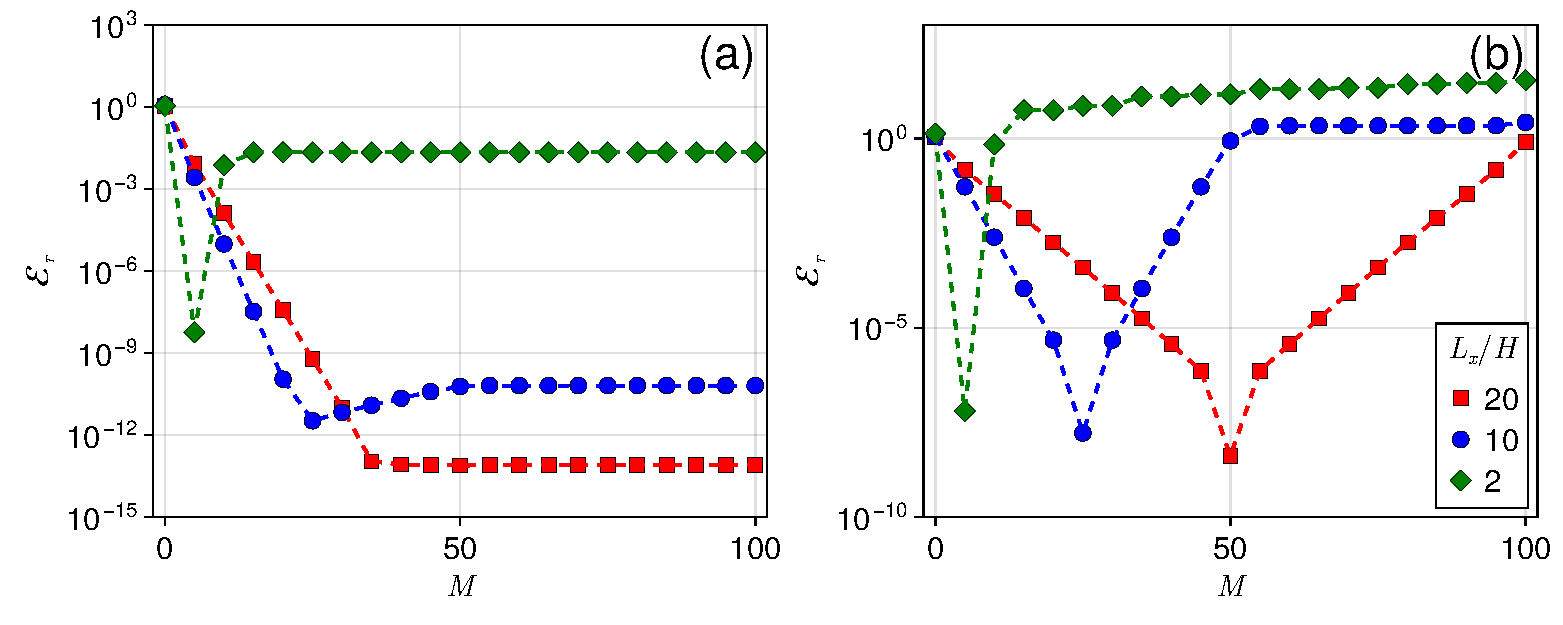
\includegraphics[width=0.98\linewidth]{figs/icm_elc_error_force.pdf}
    \caption{Relative error of force ($\mathcal{E}_r$) in a dielectric-confined Coulomb system with parameters $R = 5$ and $H = 0.5, 1, 5$. In panels (a) and (b), the dielectric contrasts are set to $\gamma_{\T u} = \gamma_{\T d} = \gamma = 0.6$ and $\gamma_{\T u} = \gamma_{\T d} = \gamma = 1$, respectively.}
    \label{fig:icm_elc_error_force}
\end{figure}

\begin{figure}[htbp]
    \centering
    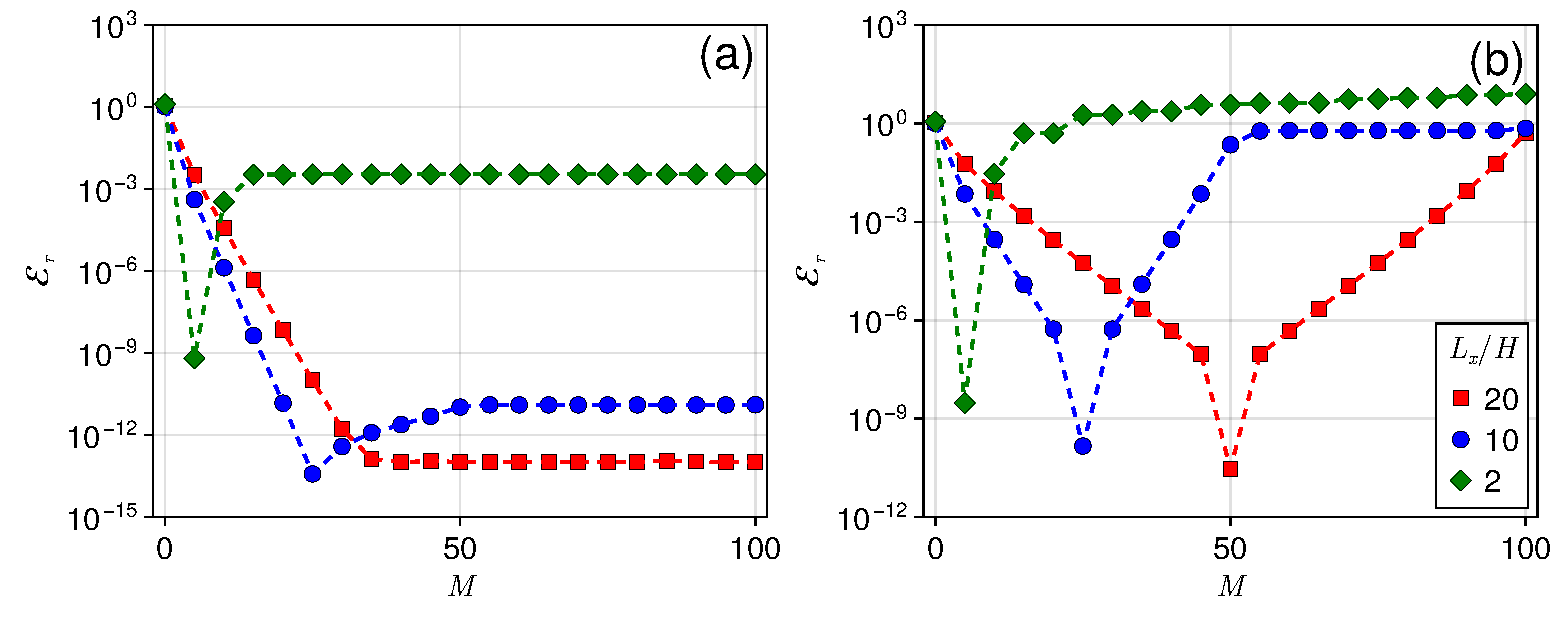
\includegraphics[width=0.98\linewidth]{figs/icm_elc_error.pdf}
    \caption{Relative error of energy in a dielectric-confined Coulomb system with parameters $P = 5$ and $H = 0.5, 1, 5$. In panels (a) and (b), the dielectric contrasts are set to $\gamma_{\T u} = \gamma_{\T d} = \gamma = 0.6$ and $\gamma_{\T u} = \gamma_{\T d} = \gamma = 1$, respectively.}
    \label{fig:icm_elc_error}
\end{figure}